
\section{Square Lattice}\label{square_lattice}

\subsubsection{Lattice Structure and DOS}

The square lattice is a relatively simple system which can help understand concepts and check algorithms before jumping to more complex systems and substrates. In two dimensions the square lattice can be constructed with two lattice vectors $\Vec{a}$ and $\Vec{b}$, such that
\begin{equation}
    \mathbf{R} = m\Vec{a} + n\Vec{b} \for n,m\in\integernumbers,
\end{equation}
is a well-defined point (see figure \ref{fig:square_lattice}). The area highlighted in red is the so-called Wigner-Seitz cell, a primitive unit cell with one lattice point \cite{Hofmann2015}. In other words, the entire square lattice can be constructed with one constant $a=||\Vec{a}||=||\Vec{b}||= \SI{2.46}{\angstrom}$. We will consider only nearest neighbour hopping, such that we can use the Hamiltonian from equation \ref{eq:reduced_hamil} with hopping parameter $t=\SI{2.7}{eV}$. For a $20\times 20$ periodic square lattice, the Hamiltonian consists of $400$ rows and $400$ columns with four hopping parameters per row. All other elements are zero. 

\begin{figure}[H]
    \centering
    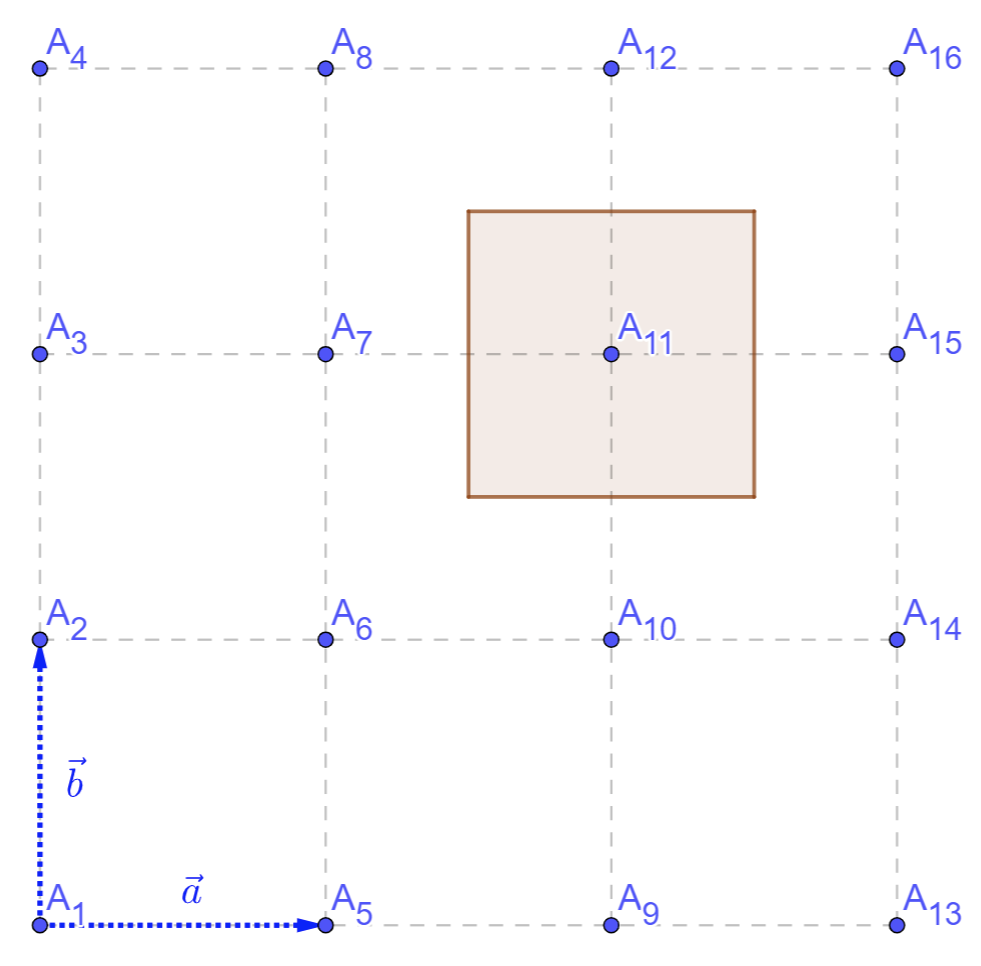
\includegraphics[width=.4\textwidth]{img/squarelattice_structure.PNG}
    \caption{Structure of a $4\times 4$ square lattice, where $\Vec{a}$ and $\Vec{b}$ are lattice constants. The highlighted area is the Wigner-Seitz cell \cite{Hofmann2015}.}
    \label{fig:square_lattice}
\end{figure}

The eigenvalues of this matrix can be used to plot the DOS (see equation \ref{eq:time_ind_schrödinger}), which is shown in figure \ref{fig:DOS_square_lattice_per} (see figure \ref{fig:DOS_square_lattice} in appendix \ref{figures} for the DOS of a non-periodic $20\times 20$ square lattice). The histogram in yellow shows the cumulative number of states that are occupied by the system within a certain energy range. The three lines show the probability of an electron having a certain eigenenergy using different smoothing parameters. Using a parameter which is too large will result in an obscured plot, such that peaks are flattened and the eigenstates are not localised (see green line in figure \ref{fig:DOS_square_lattice_per}). Using a parameter which is too small will result in an distorted plot (see red line in figure \ref{fig:DOS_square_lattice_per}). In this case the eigenstates are assumed to be very localised, which can make it very difficult to interpret the plot for the DOS. For the DOS of the $20\times 20$ square lattice it seems like a smoothing parameter of $h=0.5$ is a suitable choice.

\begin{figure}[H]
    \centering
    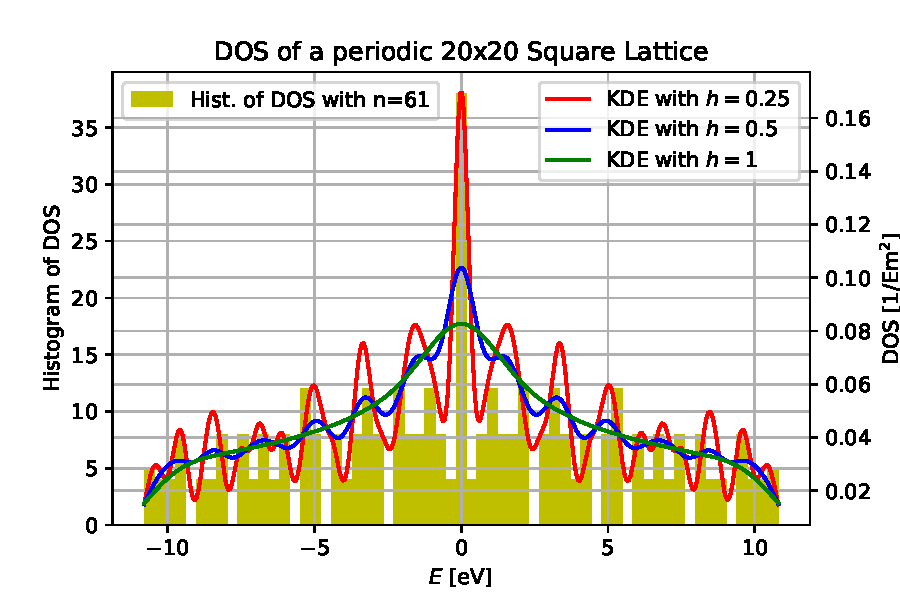
\includegraphics[width=.7\textwidth]{img/DOS_20x20_square_lattice_per.pdf}
    \caption{Density of states of a $20\times 20$ periodic square lattice with different smoothing parameters $h$. The left axis shows the cumulative number of eigenstates $E$ within the total range $[E_{min},E_{max}]$ divided over a certain number of bins (here $n=61$ bins), whereas the right axis corresponds to the KDE of the DOS (see section \ref{density_of_states}).}
    \label{fig:DOS_square_lattice_per}
\end{figure}

\subsubsection{Description of Plasmonic Excitations}

The Coulomb interaction matrix for the square lattice is given by the classical potential (see equation \ref{eq:classical_coul}). From the tight binding Hamiltonian it is possible to derive the polarisability matrix $\Pi$ with the random phase approximation \cite{Westerhout2018}. The polarisability combined with the Coulomb interaction defines the dielectric function, with which we can determine the EELS and the plasmon eigenmodes. In figure \ref{fig:sl_eels} we can see the EELS of a $20\times20$ square lattice and figure \ref{fig:sl_eig} shows the corresponding eigenmodes to three of the peaks in the EELS. The coefficient $d$ is a damping factor, which can be tuned to obtain better plots for the EELS (see appendix \ref{damping} for more details on the damping factor). The peaks in the spectrum correspond to plasmon frequencies \cite{Westerhout2018}.

\begin{figure}[H]
\centering
\begin{subfigure}[b]{0.7\textwidth}
   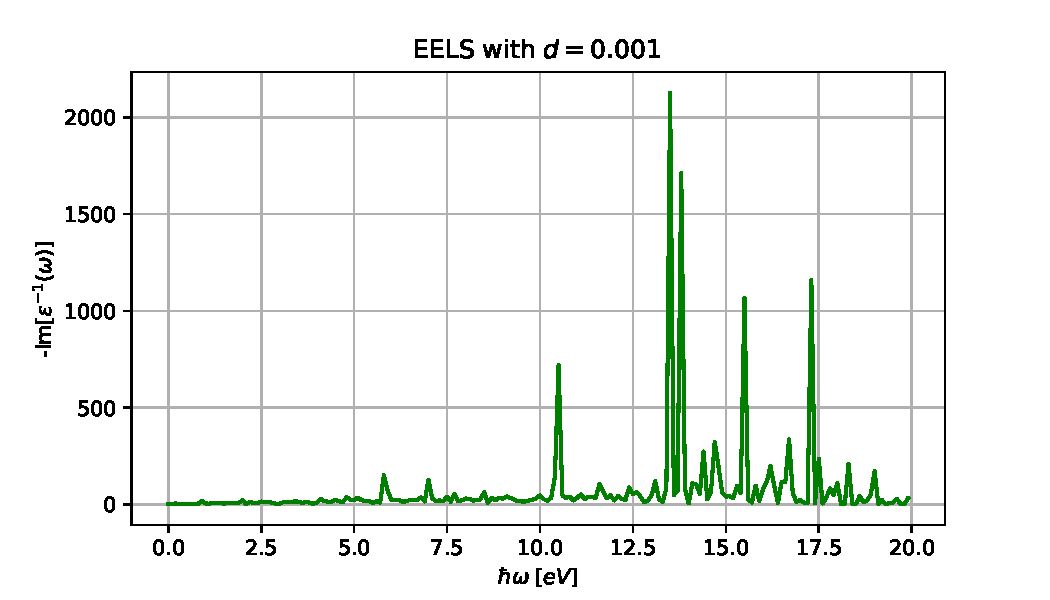
\includegraphics[width=1\linewidth]{img/square_lattice_eels.pdf}
   \caption{}
   \label{fig:sl_eels} 
\end{subfigure}
\begin{subfigure}[b]{1\textwidth}
   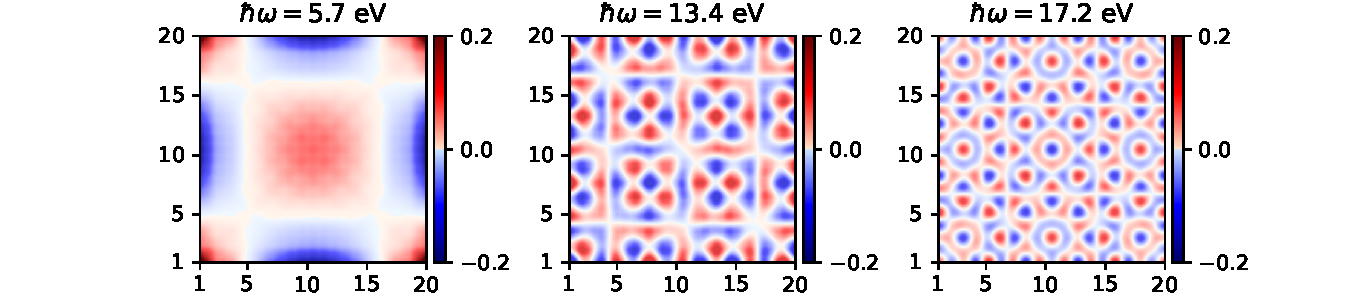
\includegraphics[width=1\linewidth]{img/square_lattice_eigenmodes.pdf}
   \caption{}
   \label{fig:sl_eig}
\end{subfigure}
\caption{(a) EELS of the $20\times20$ periodic square lattice with a damping factor of $d=\SI{0.001}{eV}$. (b) Three different plasmon eigenmodes for the frequencies $\hbar\omega_1 = 5.7\mathrm{eV}$, $\hbar\omega_2 = 13.4\mathrm{eV}$, $\hbar\omega_3 = 17.2\mathrm{eV}$. The x- and y-axis denote a lattice point in the $20\times20$ periodic square lattice and the colour-bar denotes the charge of the plasmonic excitations (blue: negative, red: positive).}
\end{figure}



%%%%%%%%%%%%%%%%%%%%%%%%%%%%%%%%%%%%



\section{Mono-Layer Graphene}\label{monolayer_graphene}

\subsection{Lattice Structure and DOS}

As mentioned in the previous section (see section \ref{square_lattice}), a two-dimensional square lattice is a relatively simple system. This is different for Graphene, which exhibits a honeycomb structure \cite{Katsnelson2020}. This structure cannot be described with primitive unit cells, which can only contain one lattice point \cite{Hofmann2015}. It is therefore necessary to define a sub-lattice, such that each (non-primitive) unit cell has two lattice points (see red highlighted area in figure \ref{fig:graphene_lattice}). The blue vectors $\Vec{a}$ and $\Vec{b}$ in figure \ref{fig:graphene_lattice} are the lattice constants between two unit cells, whereas the vector $\Vec{c} = \frac{1}{3}\Vec{a}+\frac{2}{3}\Vec{b}$ is the translation between the two sub-lattices (blue and red dots). Note that the unit cell can be constructed differently (e.g. connecting the dots $B_1$, $B_5$, $B_8$, $B_4$), which will result in an equivalent definition of the lattice \cite{Hofmann2015}. In figure \ref{fig:graphene_snowflake} we can see how this looks like for a small system with $n=366$ lattice points. The density of states of this graphene lattice is given in figure \ref{fig:DOS_graphene}, where we can see why graphene is referred to as a zero-gap semiconductor (also referred to as gap-less semiconductor or semimetal) \cite{Radamson2017}. Normally semiconductors, like silicon, show a band gap around the Fermi energy and metals do not possess a gap, i.e. the DOS assumes finite values at Fermi energy \cite{Radamson2017}. 

\begin{figure}[H]
\centering
\begin{subfigure}[b]{.54\textwidth}
  \centering
  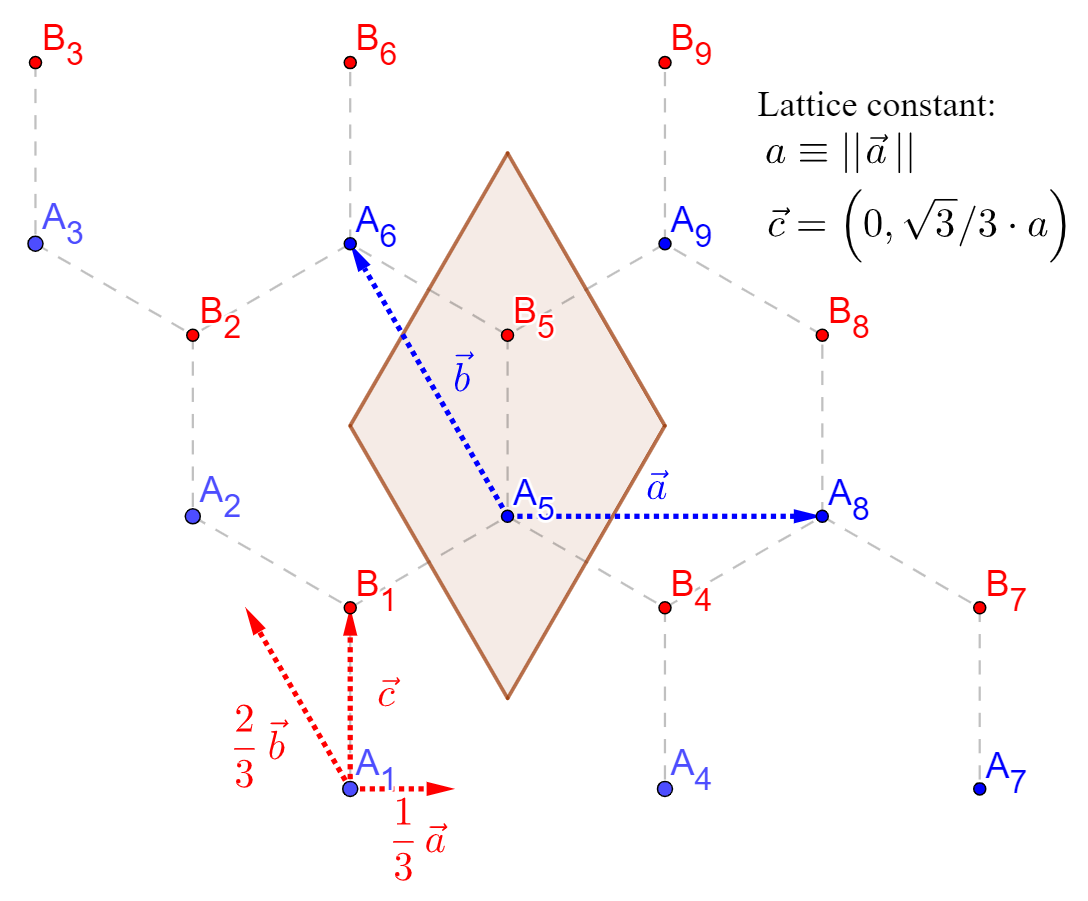
\includegraphics[width=\textwidth]{img/graphene_structure_1.PNG}
  \caption{}
  \label{fig:graphene_lattice}
\end{subfigure}
\hfill
\begin{subfigure}[b]{.45\textwidth}
  \centering
  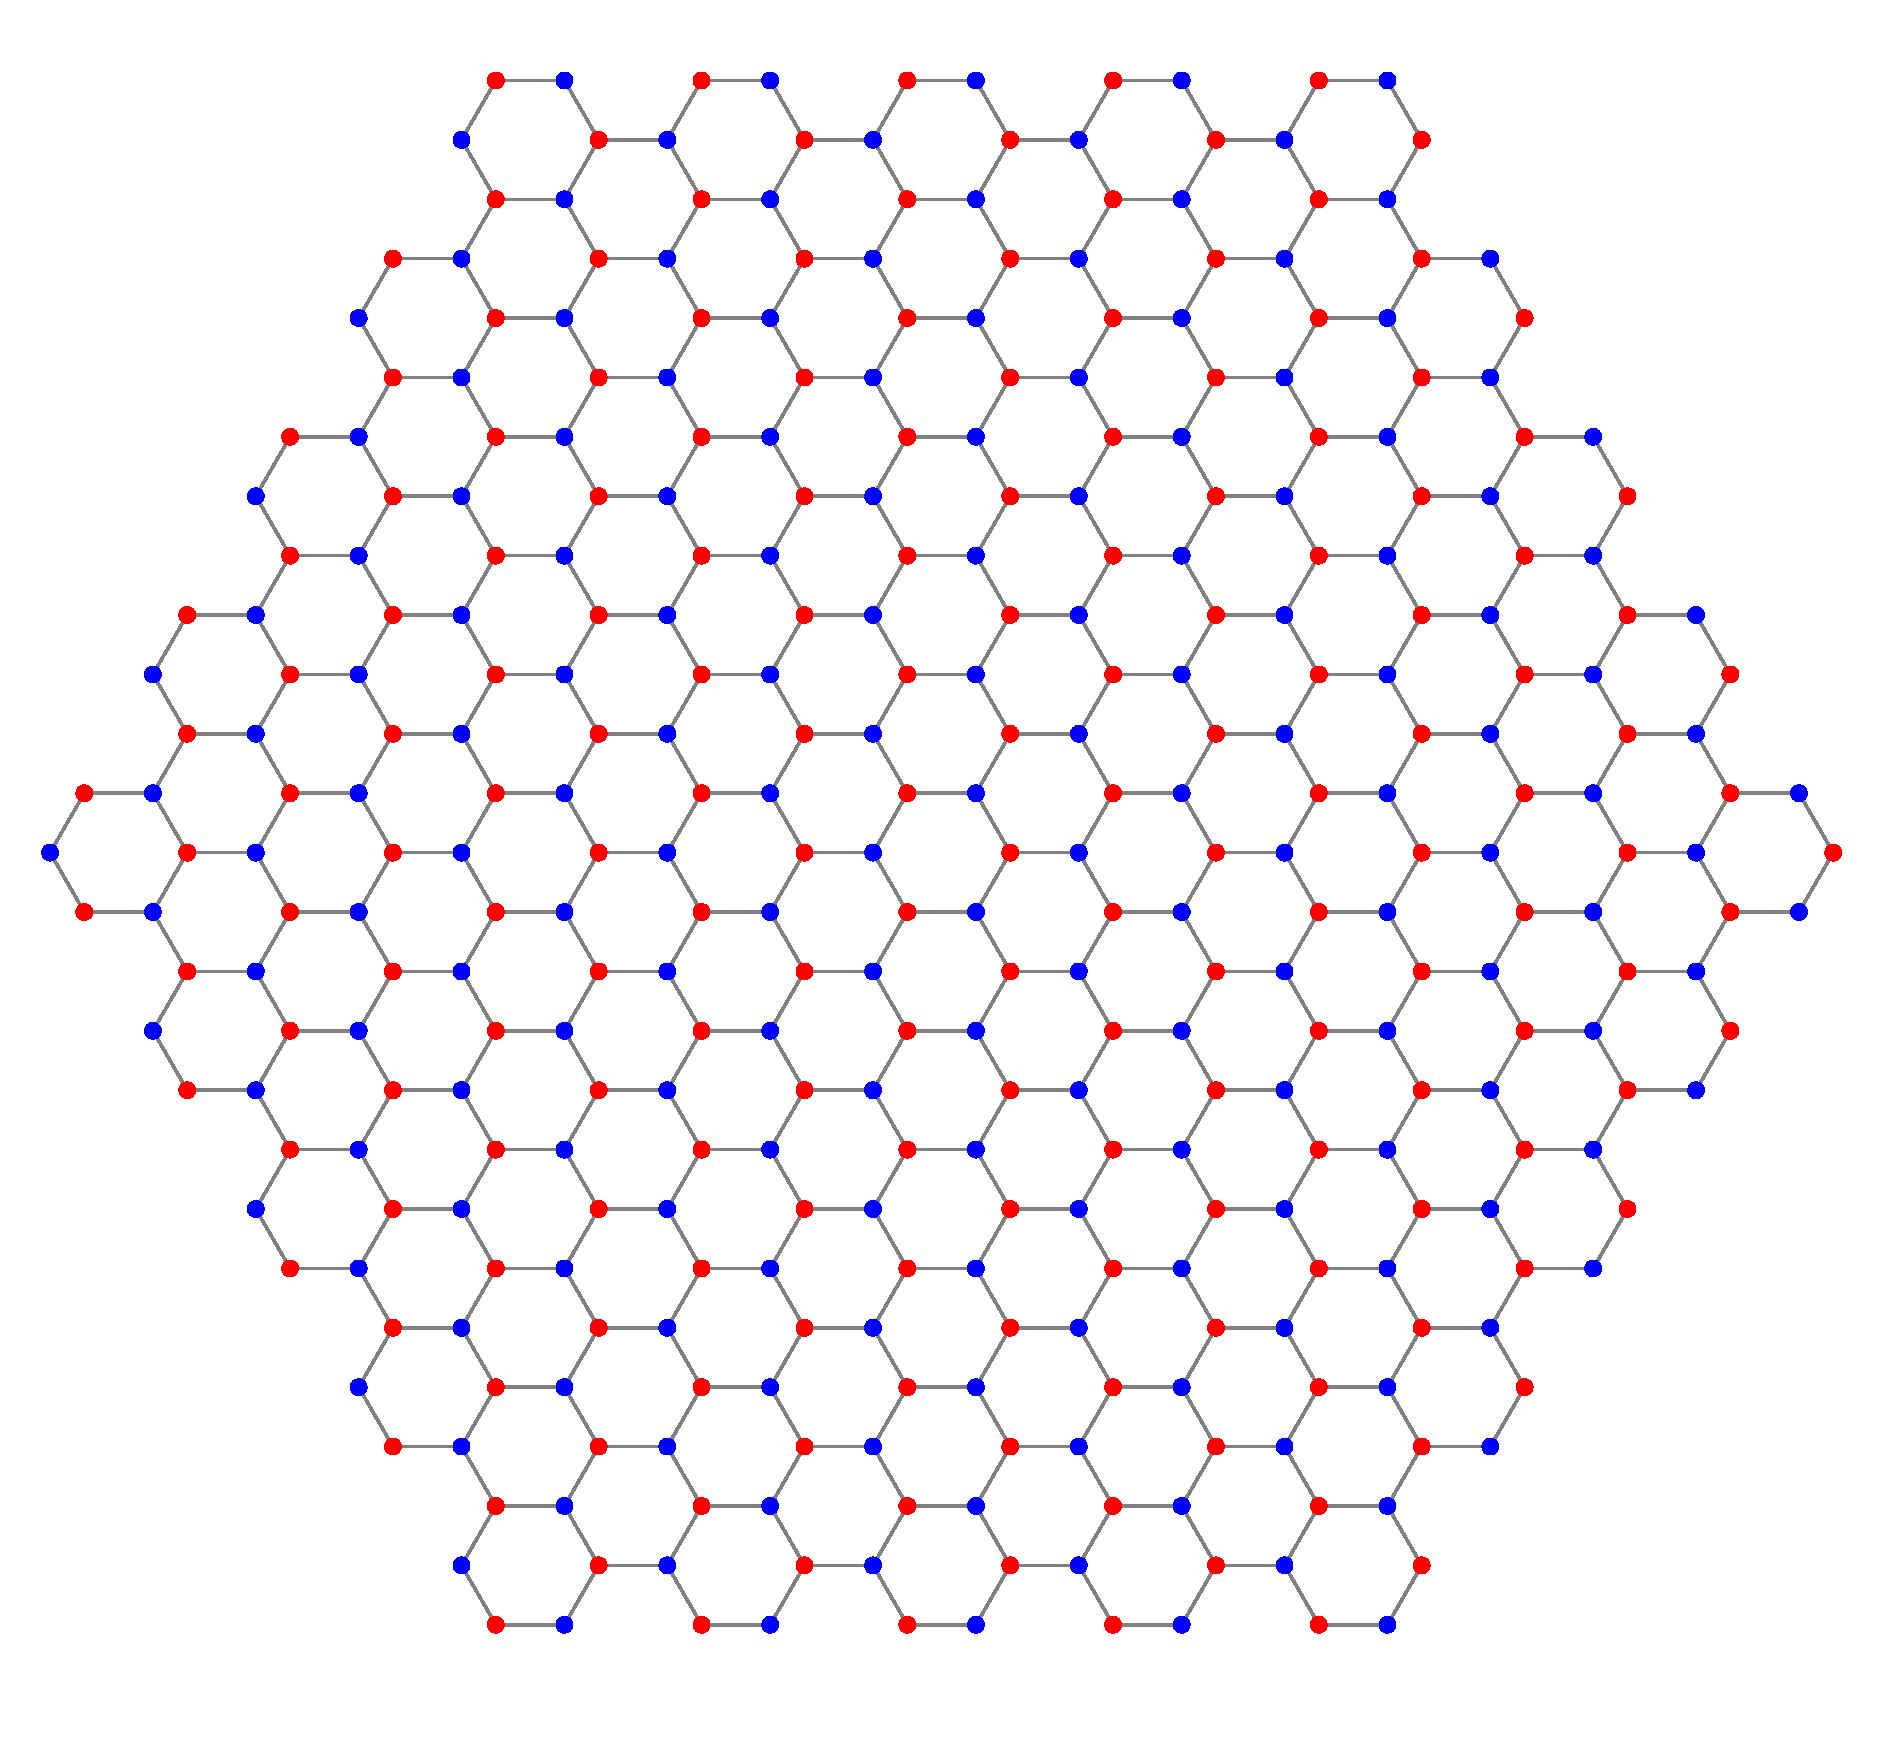
\includegraphics[width=\textwidth]{img/snowflake_subsample_sketch.pdf}
  \caption{}
  \label{fig:graphene_snowflake}
\end{subfigure}
\caption{(a) Structure of a graphene honeycomb lattice, where $\Vec{a}$, $\Vec{b}$ are unit vectors (blue) between non-primitive unit cells (red highlighted area) and the red vectors denote the transformation vectors between the unit cells and the corresponding sub-lattice (red and blue dots $A_i$, $B_i$) \cite{Hofmann2015}. (b) Graphene lattice in a snowflake-like shape with one red and one blue dot forming one unit cell. All red (or blue) dots form a sub-lattice.}
\end{figure}

\begin{figure}[H]
    \centering
    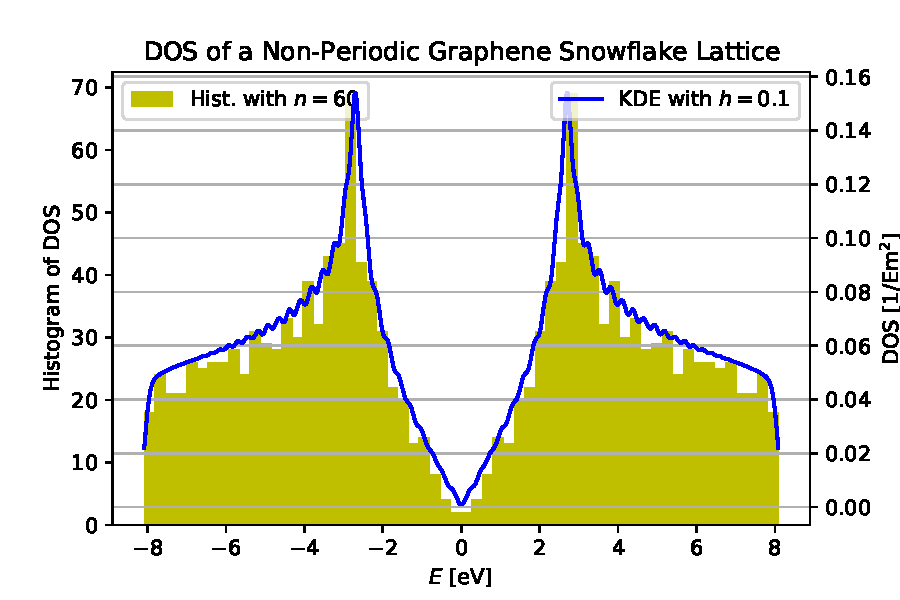
\includegraphics[width=.6\textwidth]{img/dos_snowflake.pdf}
    \caption{Density of states of a non-periodic graphene snowflake with smoothing parameters $h=0.1$ and a total of 1626 lattice points. The left axis shows the cumulative number of eigenstates $E$ within the total range $[E_{min},E_{max}]$ divided over a certain number of bins (here $n=60$ bins), whereas the right axis corresponds to the KDE of the DOS.}
    \label{fig:DOS_graphene}
\end{figure}

%%%%%%%%%%%%%%%%%%%%%%%%%%%%%%%%%%%%%%%%%%%

\subsection{Free-Standing Graphene}

\subsubsection{Coulomb Interaction}

The Coulomb interaction in mono-layer graphene can be determined using ab initio cRPA calculations. This has been done for a rhombus-shaped graphene lattice with unit cell constant $a = \SI{2.468032}{\angstrom}$ and periodic boundary conditions. In figure \ref{fig:ab_initio_coul} we can see the ab initio data for the Coulomb interaction between all lattice points. The Coulomb elements from the ab initio data grow as $r$ increases, which is a consequence of periodic boundary conditions. These boundary conditions imply that two points on opposite sides of the lattice are treated as nearest neighbours, which creates a vertical symmetry (see figure \ref{fig:ab_initio_coul}). As we will be fitting this data to the model given in equation \ref{eq:cho} for distances smaller than $\SI{10}{\angstrom}$, the boundary conditions and the shape of the lattice should not have a big impact on the Coulomb interaction and can therefore be neglected. The blue dots in figure \ref{fig:ab_initio_coul} denote the interaction between the initial points of the unit cells (A-A) and the blue dots the interaction between the two sub-lattices (see blue and red points in figure \ref{fig:graphene_lattice}).

The cyan line in figure \ref{fig:fsg_cho} shows the classical Coulomb interaction given in equation \ref{eq:classical_coul} and we can immediately see why the classical model is not suitable to describe mono-layer graphene. The nearest neighbour interaction is overestimated in the classical model. By fitting the cRPA data to the function $U(r)$ given in equation \ref{eq:cho}, we will obtain the purple line shown in figure \ref{fig:fsg_cho}. The ab initio data for $r<\SI{10}{\angstrom}$ is shown in green. We can see that this function fits the data points incredibly well, including the nearest neighbour interaction and the on-site interaction. This Coulomb model is therefore suitable to determine the dielectric function for a non-periodic snowflake lattice via the RPA. For a thickness\footnote{With thickness we define the distance between the layers $\epsilon_2$ and $\epsilon_3$, which in the case of free-standing graphene are $\epsilon_2=\epsilon_3 =\epsilon_0=\SI{1}{eV}$} $d = \SI{3.35}{\angstrom}$ we were able to find the following values for $\delta$ and $\epsilon_1$:
\begin{equation}\label{eq:params_FSG}
    \delta = \SI{0.70901644}{\angstrom} \aand \epsilon_1= 2.57524703
\end{equation}

\begin{figure}[H]
\centering
\begin{subfigure}[b]{.49\textwidth}
  \centering
  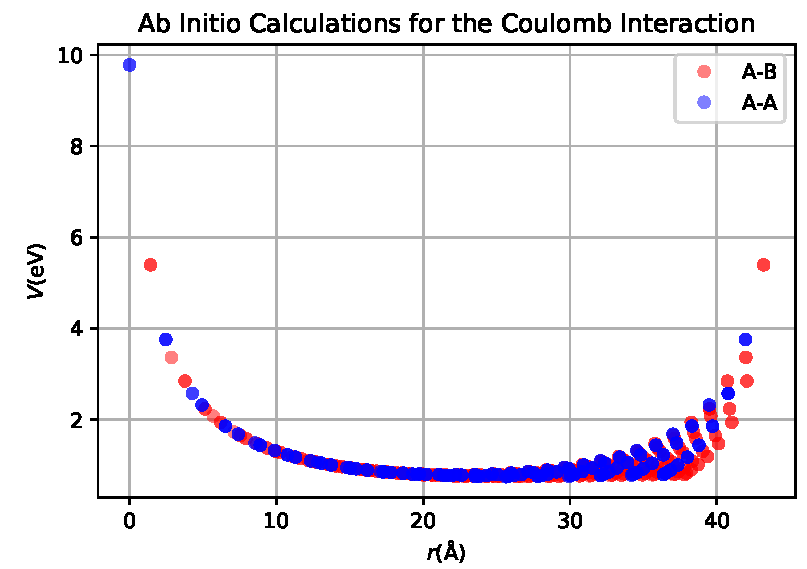
\includegraphics[width=\textwidth]{img/ab_initio_coul.pdf}
  \caption{}
  \label{fig:ab_initio_coul}
\end{subfigure}
\begin{subfigure}[b]{.49\textwidth}
  \centering
  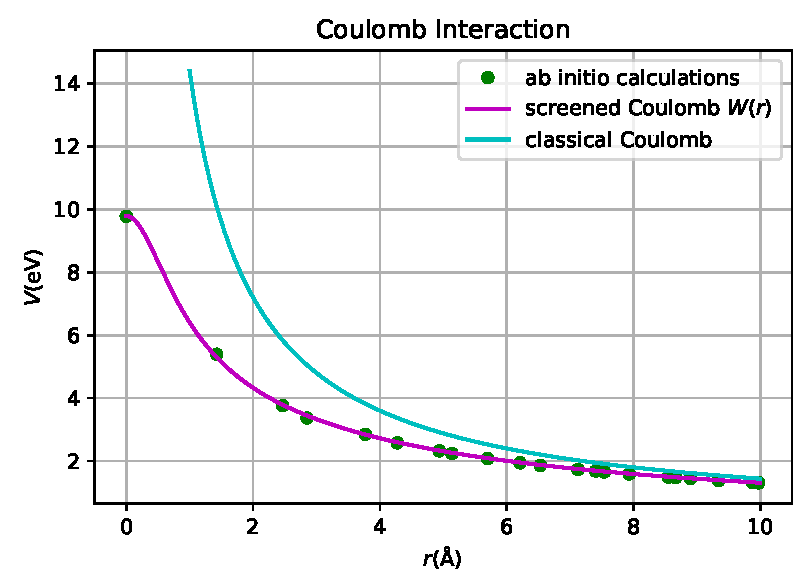
\includegraphics[width=\textwidth]{img/FSG_Cho_2018.pdf}
  \caption{}
  \label{fig:fsg_cho}
\end{subfigure}
\caption{(a) Coulomb interaction in free-standing graphene, where the red and blue dots represent the ab initio data of the two sub-lattices. (b) The green dots are the ab initio data for $r<\SI{10}{\angstrom}$, the purple line is the screened Coulomb potential given in equation \ref{eq:cho} fitted to the ab initio data and and the cyan line is the classical Coulomb interaction (see equation \ref{eq:classical_coul}).}
\end{figure}

%%%%%%%%%%%%%%%%%%%%%%%%%%%%%%%%%%%%%%%

\subsubsection{Description of Plasmonic Excitations}

The total energy loss function of the electrons is shown in figure \ref{fig:damp_comp} (see appendix \ref{damping}) for a large frequency-range of $\omega \in \abrackets{0,5}\mathrm{eV}$. We will now analyse the lower frequencies, especially the infrared spectrum and the low frequency visible spectrum (red light), i.e. a frequency-range of $\omega \in\abrackets{0,2}\mathrm{eV}$ \cite{Serway2014}, because the plasmonic excitations where we have extremely localised surface charge density oscillations, are expected to be within this range. In section \ref{plasmonic_excitations} we mentioned that the dielectric function $\epsilon(\omega)$ (see equation \ref{eq:dielectric}) equals zero if it corresponds to a plasmon frequency. A way to find plasmon frequencies is to determine the EELS and find its maxima. On top of that the dielectric function corresponding to these maxima must fulfil the condition \cite{Westerhout2018}
\begin{equation}\label{eq:realpart_cond}
    \re(\epsilon(\omega))=0 \aand \re(\epsilon(\omega_1))<\re(\epsilon(\omega_2)) \for \omega_1<\omega<\omega_2.
\end{equation}
In other words the dielectric function of a plasmon frequency has a real part which both equals zero and is increasing \cite{Westerhout2018}. In figure \ref{fig:eels_fsg_s1} we can see the real part of the dielectric function as a blue dotted line and the EELS as a green line. The red vertical line denotes the frequency where the blue line fulfils the conditions given in equation \ref{eq:realpart_cond}. We can see that the peak of the EELS can be found at approximately the same height as the vertical line, which is a strong indicator that we are dealing with a plasmonic excitation. The plasmon frequency is $\hbar\omega = \SI{0.8157}{eV}$ and the eigenmode corresponding to this frequency is shown in figure \ref{fig:eigenmode_fsg_s1}. We are dealing with a total of 1626 lattice points, which means that the length of the hexagon is approximately $\SI{40}{\angstrom}$.

\begin{figure}[H]
\centering
\begin{subfigure}[b]{.55\textwidth}
  \centering
  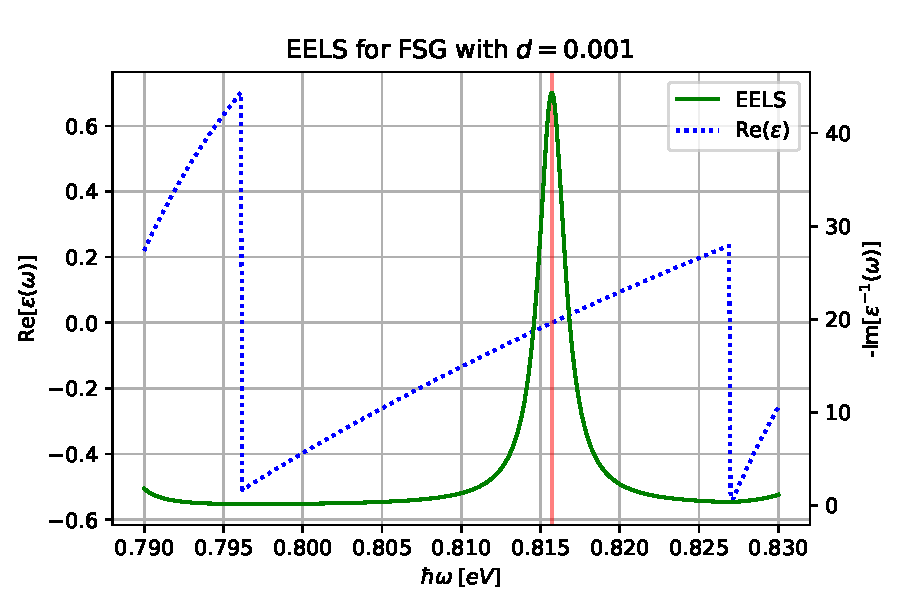
\includegraphics[width=\textwidth]{img/eels_FSG_059-061.pdf}
  \caption{}
  \label{fig:eels_fsg_s1}
\end{subfigure}
\hfill
\begin{subfigure}[b]{.44\textwidth}
  \centering
  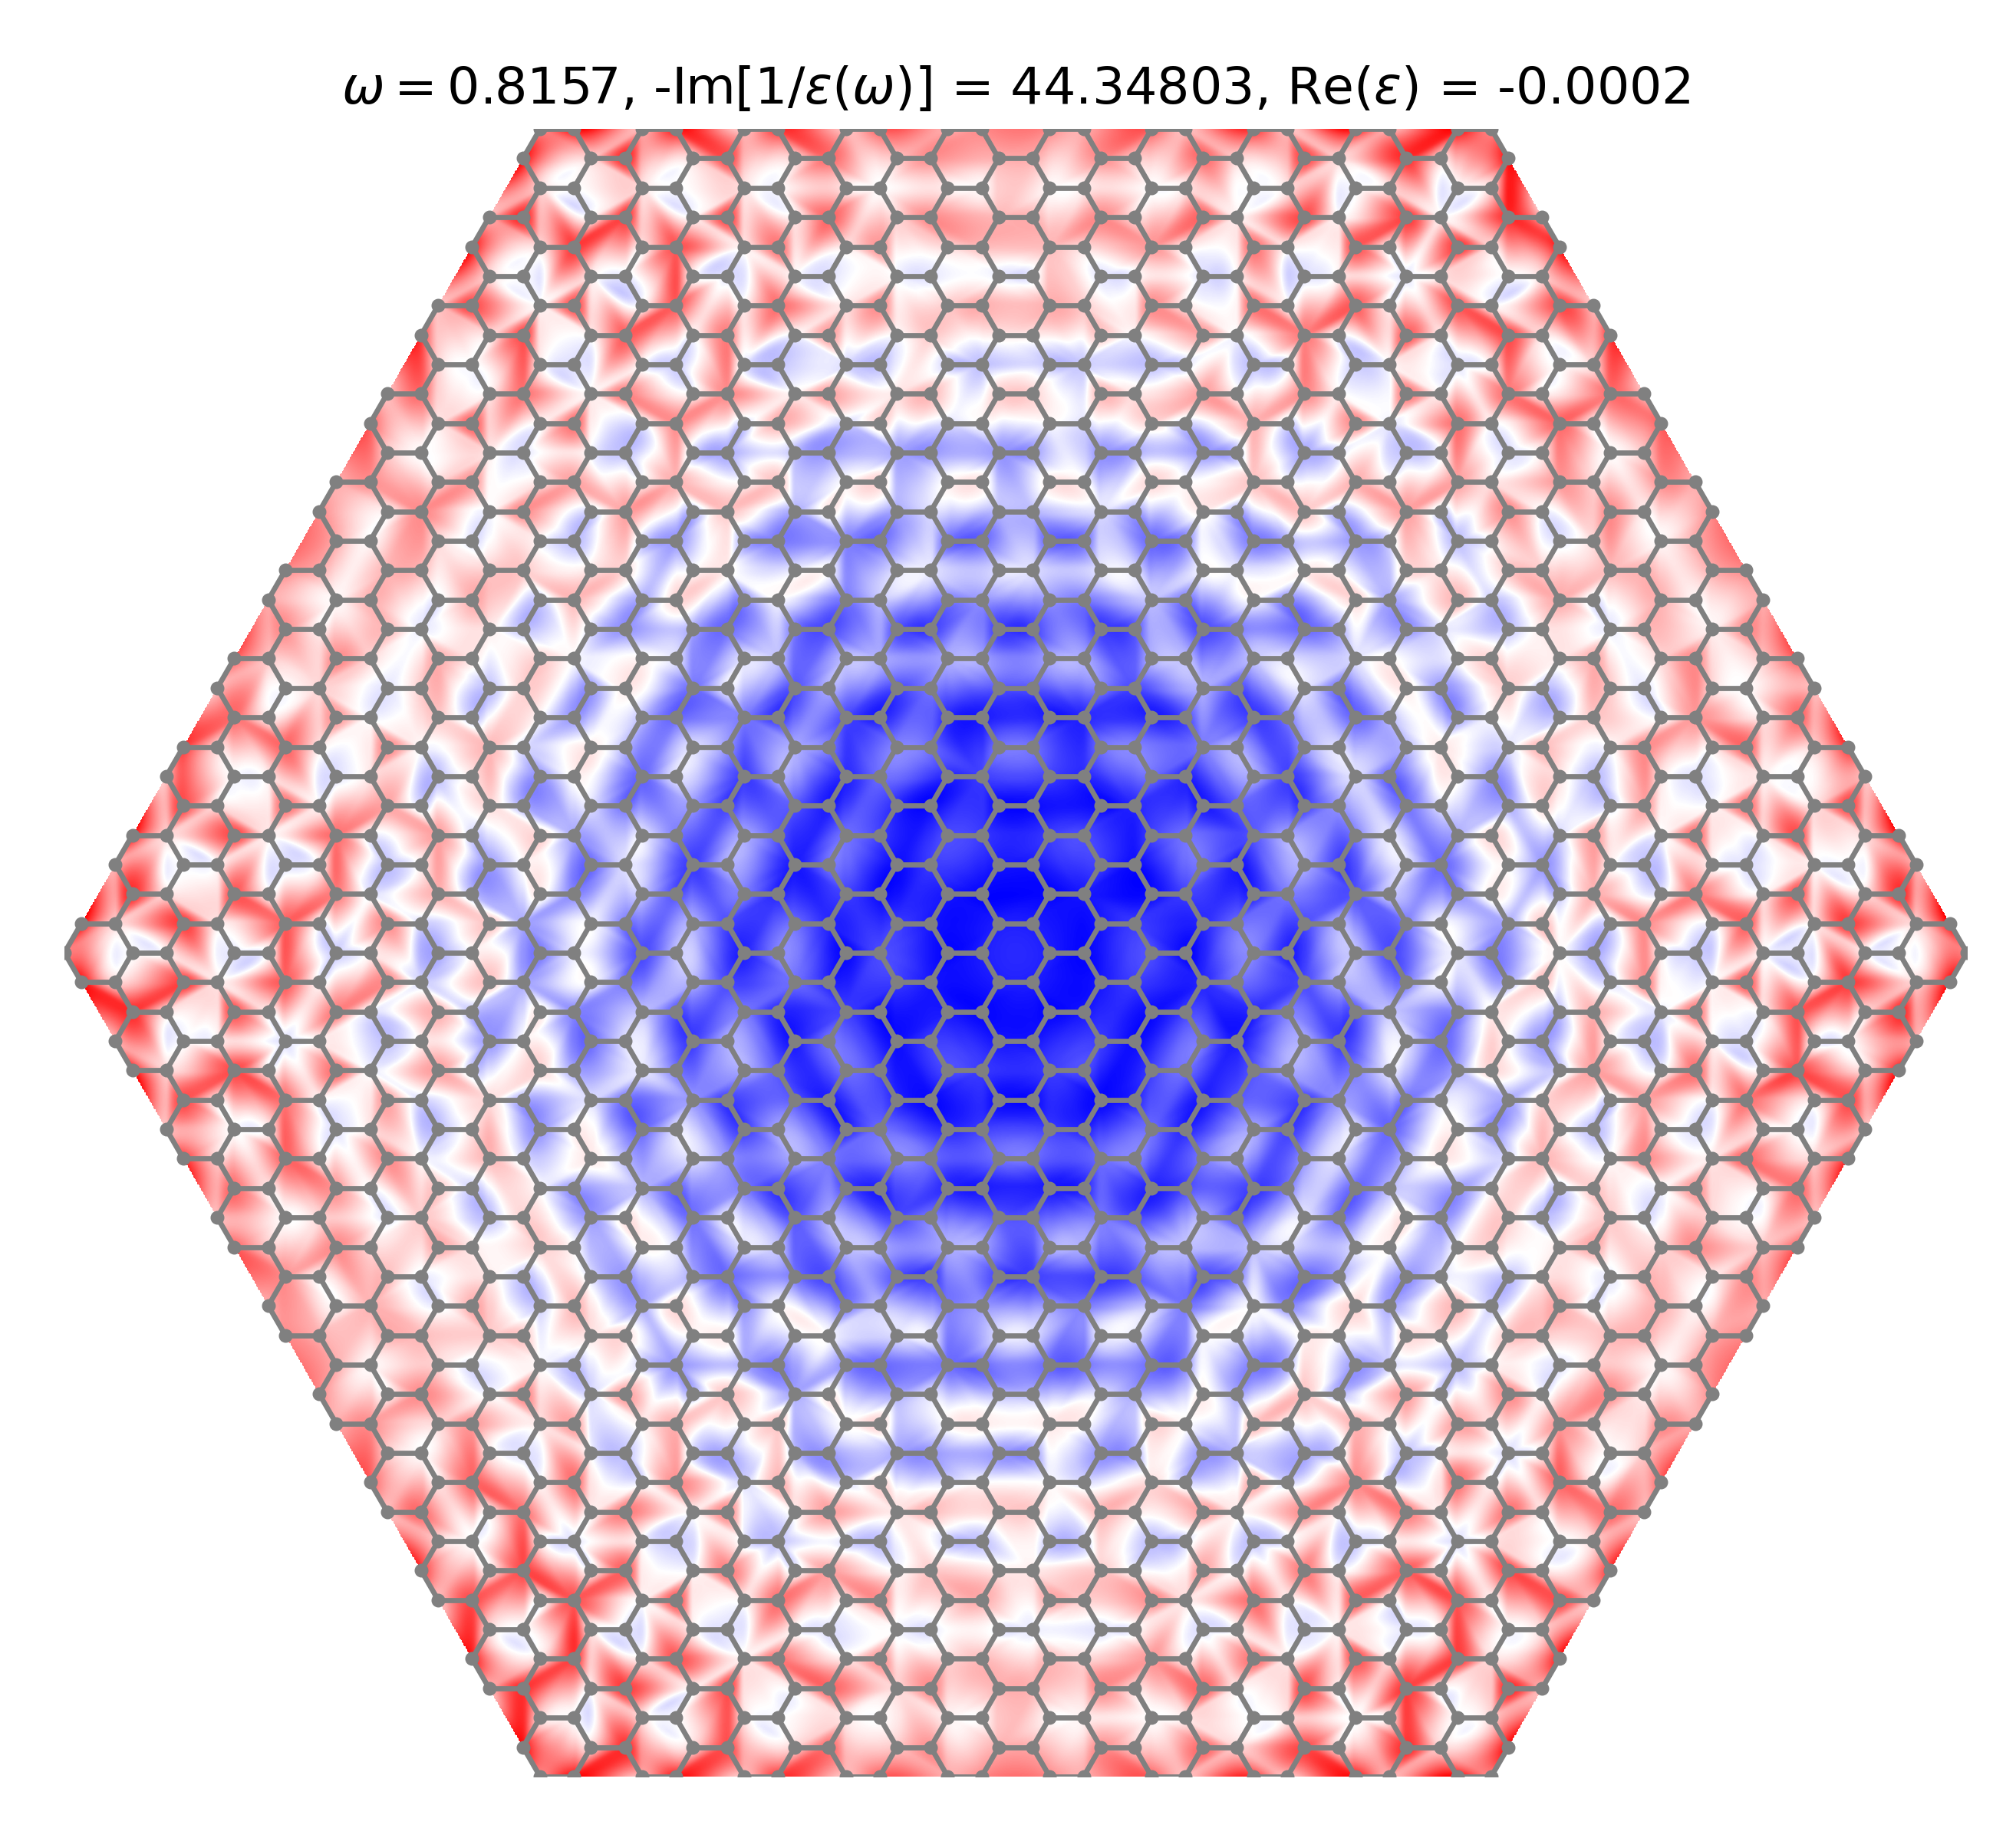
\includegraphics[width=\textwidth]{img/mg_plasmons_0.8157.png}
  \caption{}
  \label{fig:eigenmode_fsg_s1}
\end{subfigure}
\caption{(a) Real (blue dots) and the imaginary (green line) part of the EELS with a vertical red line indicating the plasmonic excitation. (b) Eigenmode corresponding to the plasmon frequency in figure \ref{fig:eels_fsg_s1}}
\end{figure}



%%%%%%%%%%%%%%%%%%%%%%%%%%%%%%%%%%%%%

\subsection{Graphene Embedded in Hexagonal Boron Nitride}\label{boron_nitride}

\subsubsection{Coulomb Interaction}

Hexagonal boron nitride (h-BN) has the same lattice structure as graphene and very similar lattice constants, which makes it a very interesting choice as a dielectric layer embedding graphene \cite{Sarma2011,Wang2017}. Research has shown that h-BN is a great substrate when it comes to retaining the electrical properties of graphene \cite{Wang2017}. Hexagonal boron nitride is an insulator, which implies that it has a larger band gap than free-standing graphene \cite{Wang2017}. If graphene is embedded in h-BN, the band gap of graphene will become larger and the Coulomb repulsion will increase \cite{Wang2017}, i.e. the total screened Coulomb interaction $U(r)$ (see equation \ref{eq:cho}) is expected to decrease (see ab initio points in figure \ref{fig:BN_coul}). Ideally we can use the parameters from the free-standing model given in equation \ref{eq:params_FSG} to fit the screened Coulomb interaction to the ab initio data for graphene embedded in h-BN. This should be possible because all we change is the environment, i.e. $\epsilon_2$ and $\epsilon_3$, but all other parameters should be unaffected by this. The parameters $\delta$, $\epsilon_1$ and $d$ are expected to depend on the properties of free-standing graphene. However, we can see in figure \ref{fig:BN_coul} (blue line) that there appears to be an overestimation of the on-site potential and the Coulomb interaction decreases too quickly for increasing distances. By fitting different parameters we were still not able to find a good fit for all data points. 

Figure \ref{fig:BN_coul_final} shows the screened Coulomb interaction when all parameters ($\delta, \epsilon_1,\epsilon_2,d$) are fitted. We can conclude that the model given in equation \ref{eq:cho} still holds for the case of graphene embedded in h-BN, but all parameters must be fitted. The resulting parameters are $\delta = \SI{0.7157705}{\angstrom}$, $\epsilon_1 = 3.11780114$, $\epsilon_2 = 1.34354999$, $d = \SI{10.65805182}{\angstrom}$, which show some interesting characteristics. The first constant which immediately catches attention is the thickness $d$. The thickness of the graphene layer has been fixed for the ab initio calculations and is therefore expected to be $d=\SI{3.35}{\angstrom}$. Somehow we can get a better fit when $d$ is more than three times as thick as mono-layer graphene. It seems like the parameter $d$ does now correspond to the total thickness of mono-layer graphene and the two h-BN layers. This assumption is supported by the derived values for the parameters $\epsilon_1$ and $\epsilon_2$. The dielectric constant of h-BN is expected to be between 1.8 and 3.3 \cite{Steinke2020, Laturia2018}. So $\epsilon_1$, which is now significantly larger than for free-standing graphene, seems to correspond to the total dielectric constant of all three layers. Furthermore, the parameter $\epsilon_2$ is significantly smaller than the expected dielectric constant for h-BN, and is quite close to the permittivity of free space ($\epsilon_2-\epsilon_0\approx0.34$). We might therefore hypothesise that fitting the parameters $\epsilon_1$ and $d$ to both the dielectric slab and mono-layer graphene, results in a better model.

\begin{figure}[H]
\centering
\begin{subfigure}[b]{.49\textwidth}
  \centering
  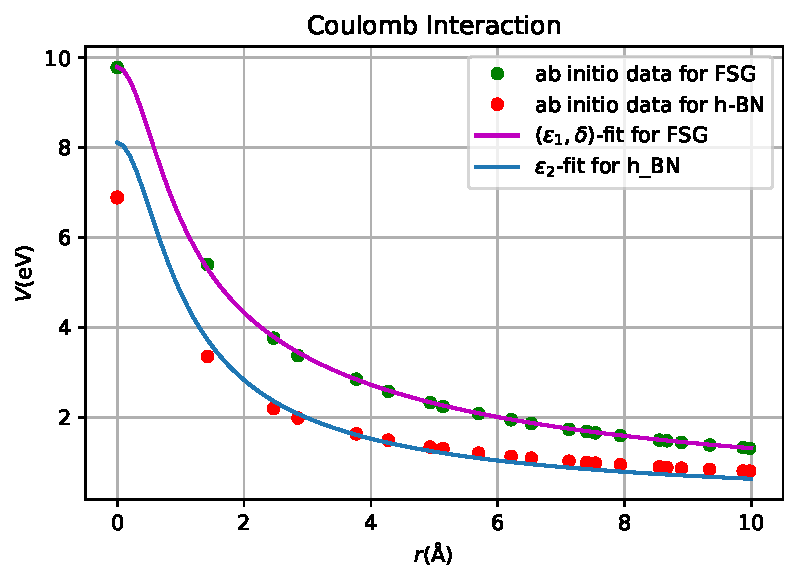
\includegraphics[width=\textwidth]{img/cho_2018_BN.pdf}
  \caption{}
  \label{fig:BN_coul}
\end{subfigure}
\hfill
\begin{subfigure}[b]{.49\textwidth}
  \centering
  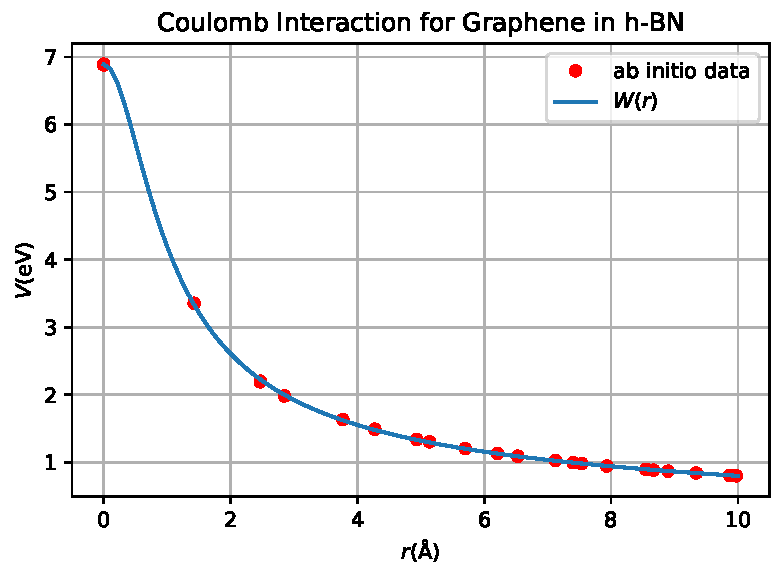
\includegraphics[width=\textwidth]{img/cho_2018_BN_all.pdf}
  \caption{}
  \label{fig:BN_coul_final}
\end{subfigure}
\caption{(a) Coulomb interaction in graphene embedded by h-BN, where the red (green) dots represent the ab initio data for h-BN (free-standing graphene). The blue (purple) line shows the fit to the ab initio data of h-BN (free-standing graphene) (b) Screened Coulomb interaction (blue line) given in equation \ref{eq:cho}, where all parameters are fitted.}
\end{figure}

%%%%%%%%%%%%%%%%%%%%%%%%%%%%%%%%%%%%%%

\subsubsection{Description of Plasmonic Excitations}

The EELS and eigenmodes can be found using the same methods we used for free-standing graphene. In figure \ref{fig:eels_bn_s1} we can see the EELS spectrum with three peaks, which correspond to plasmonic excitations. This becomes clear when looking at the red vertical lines which fulfil the conditions in equation \ref{eq:realpart_cond}. The largest of the three peaks corresponds to the $1s$-like eigenmode shown in figure \ref{fig:eigenmode_bn_s1}. It is interesting to see that the frequency which corresponds to the $1s$-like state ($\hbar\omega = 0.7915\mathrm{eV}$) has shifted to the left compared to the free-standing graphene case, where $\hbar\omega = 0.8157\mathrm{eV}$. We will investigate the shift of these frequencies in the following section.

\begin{figure}[H]
\centering
\begin{subfigure}[b]{.55\textwidth}
  \centering
  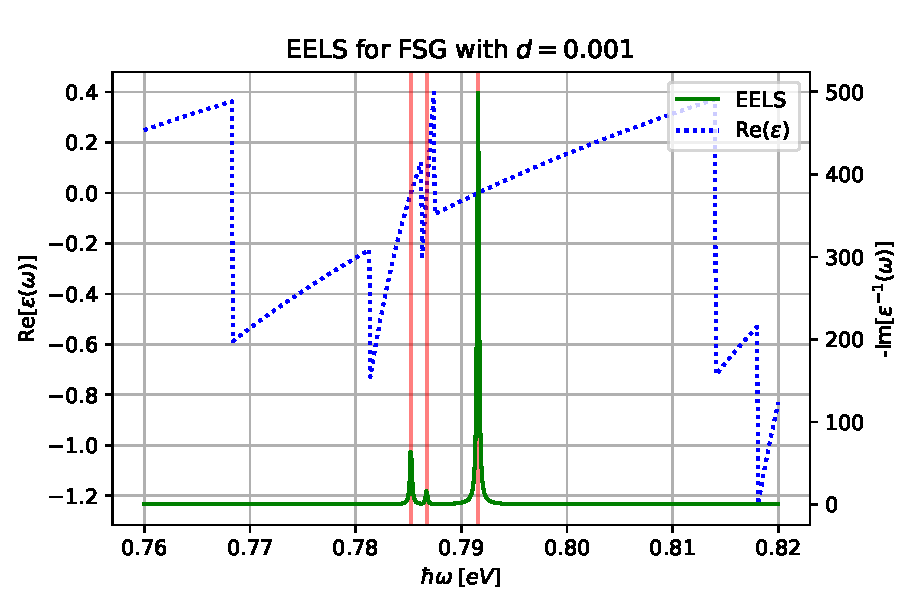
\includegraphics[width=\textwidth]{img/eels_BN_076-082.pdf}
  \caption{}
  \label{fig:eels_bn_s1}
\end{subfigure}
\hfill
\begin{subfigure}[b]{.44\textwidth}
  \centering
  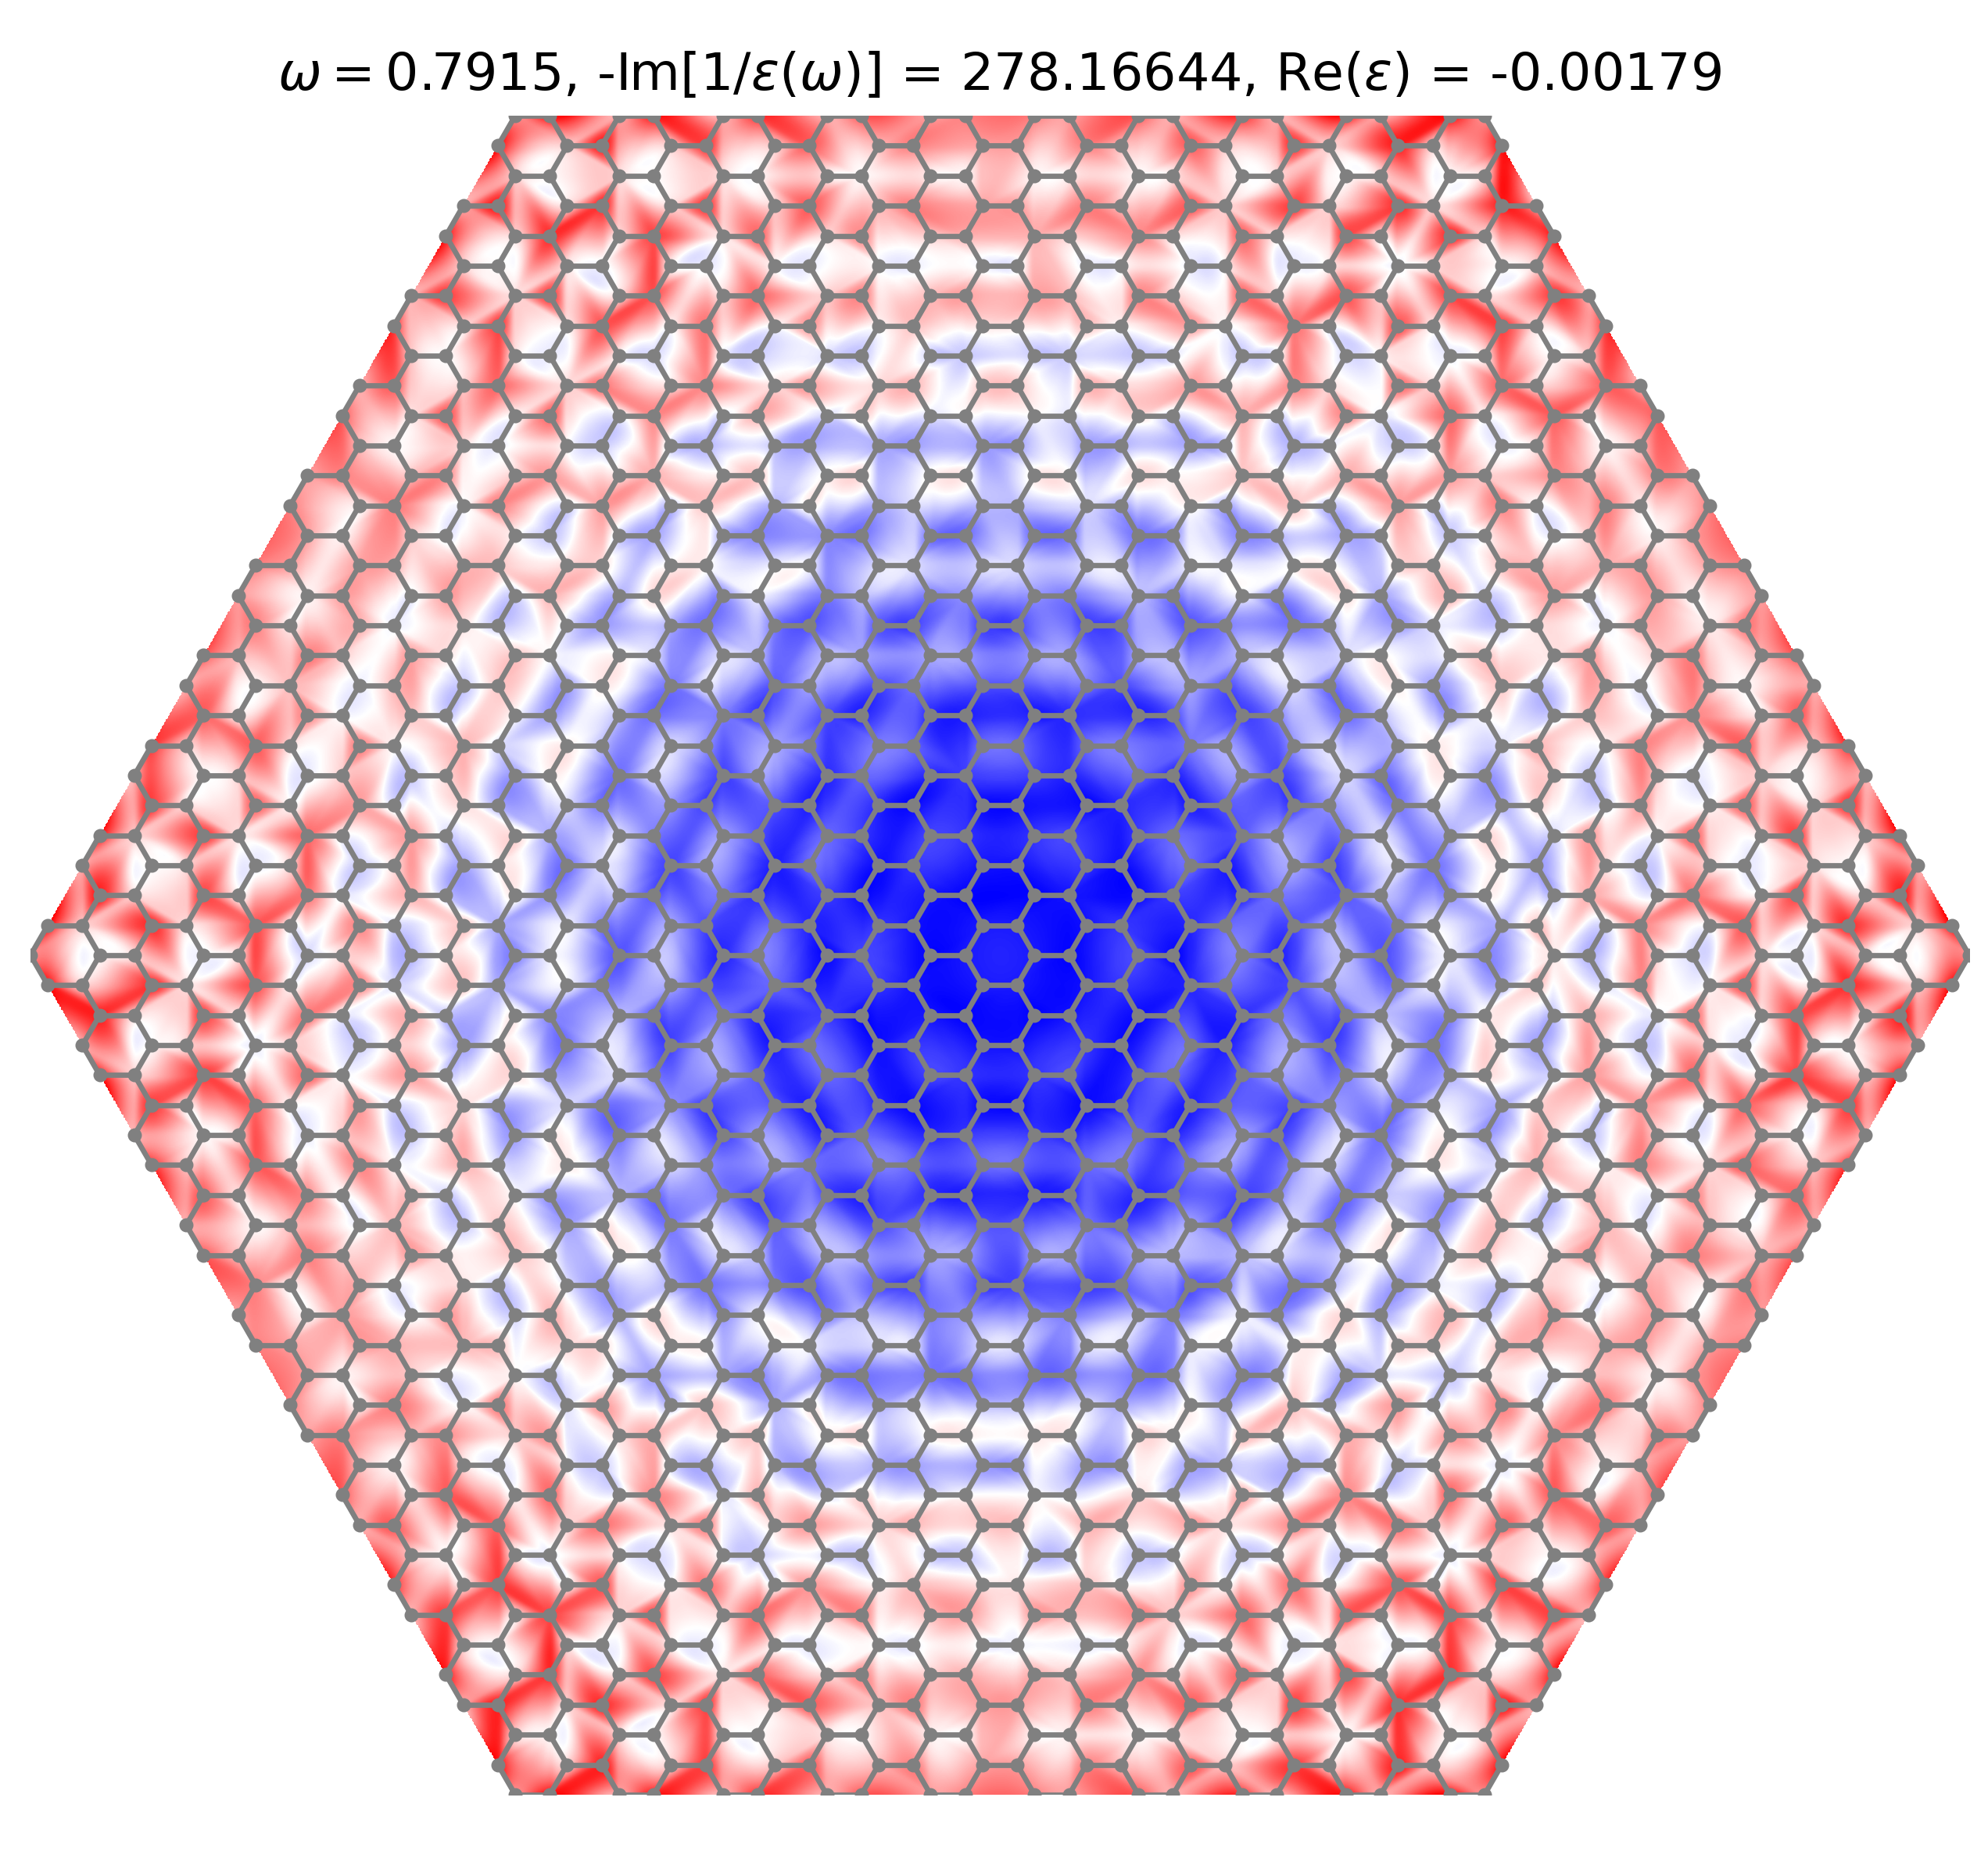
\includegraphics[width=\textwidth]{img/bn_plasmons_0.7915.png}
  \caption{}
  \label{fig:eigenmode_bn_s1}
\end{subfigure}
\caption{(a) Real (blue dots) and the imaginary (green line) part of the EELS with a vertical red lines representing the plasmonic excitations. (b) Eigenmode corresponding to the plasmon frequency in figure \ref{fig:eels_bn_s1}.}
\end{figure}



%%%%%%%%%%%%%%%%%%%%%%%%%%%%%%%%%%%%%%%

\subsection{Plasmonic Excitations in Different Dielectric Environments}\label{different_dielectric}

Previous research \cite{Steinke2020} has shown that the dielectric function $\epsilon(\omega)$ can be slightly shifted for different materials. \textcite{Steinke2020} have compared different mono-layer TMDCs\footnote{TMCD: semiconducting transition-metal dichalcogenide} affected by different dielectric surroundings. The four two-dimensional materials investigated were Tungsten disulfide $\mathrm{WS_2}$, Tungsten diselenide $\mathrm{WSe_2}$, Molybdenum disulfide $\mathrm{MoS_2}$ and Molybdenum diselenide $\mathrm{MoSe_2}$. For all four materials the absolute and the relative band-gab difference decreases for increasing dielectric constants corresponding to the substrate \cite{Steinke2020}. In figures \ref{fig:1s}-\ref{fig:1d} we can see how the frequency corresponding to a plasmonic excitation changes for different dielectric constants $\epsilon_2=\epsilon_3$\footnote{Note that the red dots in figures \ref{fig:1p} and \ref{fig:1d}, i.e. the plasmon frequencies, correspond to the $1p$- and $1d$-like eigenmodes. These eigenmodes are slightly rotated for different $\epsilon_2$. In other words, not all frequencies correspond to the eigenmode shown in the image, but to an eigenmode which is slightly rotated. The eigenmodes in figures \ref{fig:1s} and \ref{fig:2s} are rotationally invariant, such that all frequencies correspond to the eigenmode shown in the figure.}. The dielectric constant for h-BN is expected to be found between $1.8$ and $3.3$ \cite{Steinke2020,Laturia2018} For the $1s$-like state given in figure \ref{fig:1s} we were able to find a plasmon frequency of $\hbar\omega\approx\SI{0.79}{eV}$ for $\epsilon_2=2$, which matches the results found for h-BN in the previous section very well (the green line corresponds to $\hbar\omega = 0.7915\mathrm{eV}$). Furthermore, the frequencies for the $1p$- (figure \ref{fig:1p}), $1d$- (figure \ref{fig:1d}) and $2s$-like states (figure \ref{fig:2s}) are all expected to correspond to a dielectric constant of $\epsilon_2 \in \abrackets{1.8,3.3}\,\mathrm{eV}$. It is possible to draw two conclusions: first of all the frequencies corresponding to plasmons are expected to decrease when the dielectric constant $\epsilon_2$ is increased. Secondly, by altering the Coulomb interaction matrix and using the same tight-binding Hamiltonian (and consequently the same polarisability matrix), we are able to find the approximate frequency of plasmonic excitations in different dielectric environments. For instance, if graphene would be embedded in Silicon dioxide ($\mathrm{SiO_2}$), which has a dielectric constant of approximately $3.6$ \cite{Steinke2020, Lemonik2012}, the $1s$-like state can be found in the range $\hbar\omega \in \abrackets{0.763, 0.774} \mathrm{eV}$.

\begin{figure}[H]
\centering
\begin{subfigure}[b]{.49\textwidth}
  \centering
  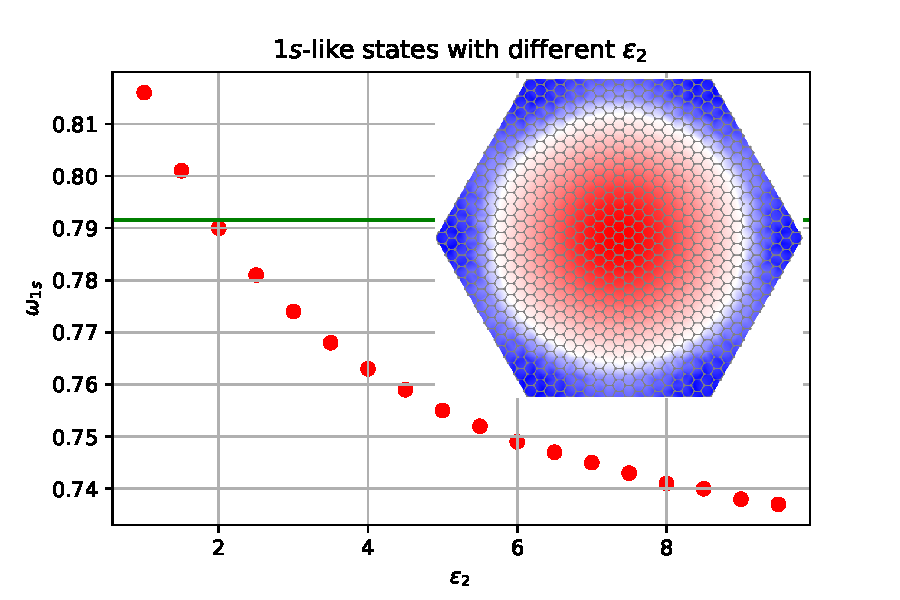
\includegraphics[width=\textwidth]{img/1s.pdf}
  \caption{}
  \label{fig:1s}
\end{subfigure}
\hfill
\begin{subfigure}[b]{.49\textwidth}
  \centering
  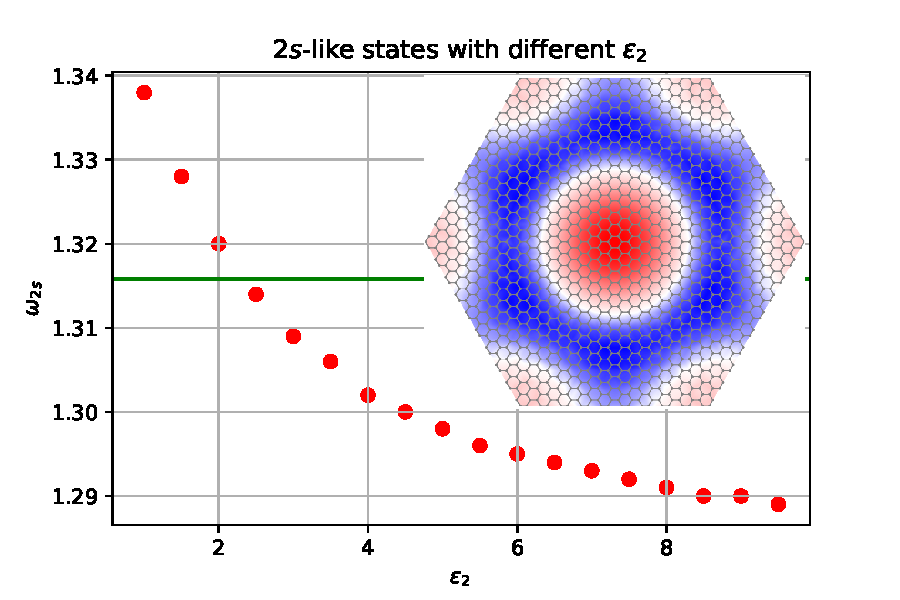
\includegraphics[width=\textwidth]{img/2s.pdf}
  \caption{}
  \label{fig:2s}
\end{subfigure}
\begin{subfigure}[b]{.49\textwidth}
  \centering
  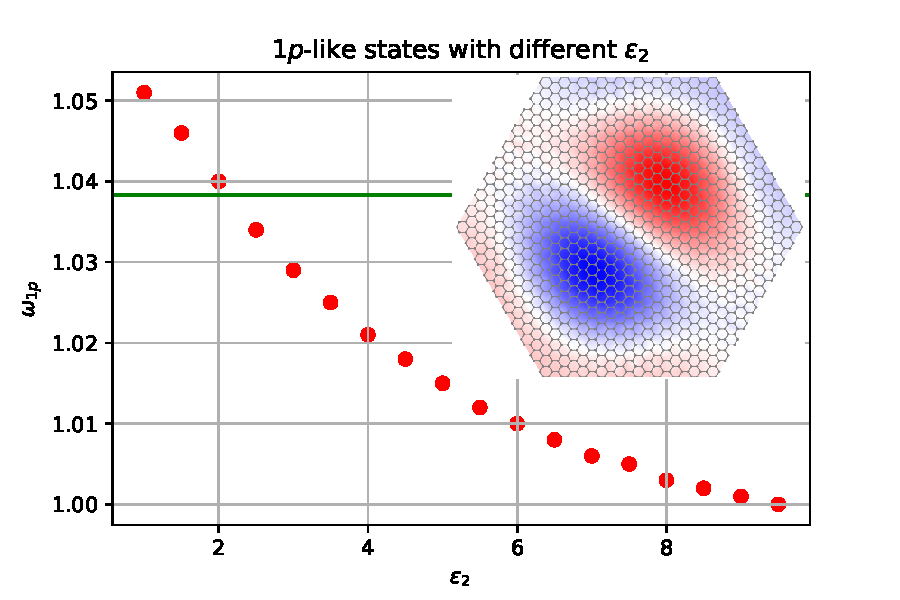
\includegraphics[width=\textwidth]{img/1p.pdf}
  \caption{}
  \label{fig:1p}
\end{subfigure}
\hfill
\begin{subfigure}[b]{.49\textwidth}
  \centering
  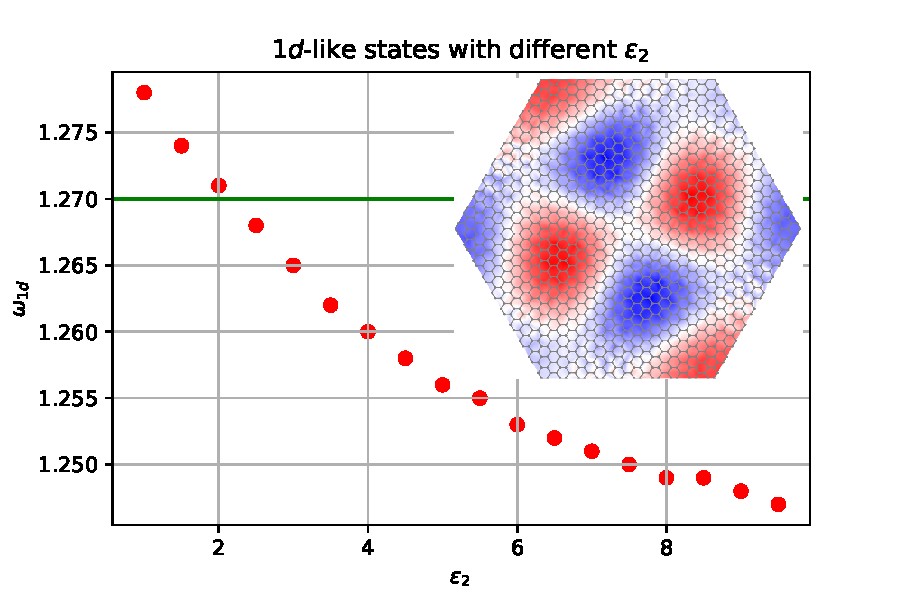
\includegraphics[width=\textwidth]{img/1d.pdf}
  \caption{}
  \label{fig:1d}
\end{subfigure}
\caption{Dependency of four different plasmon eigenmodes ($1s$-like state in \ref{fig:1s}, $2s$-like state in \ref{fig:2s}, $1p$-like state in \ref{fig:1p} and $1d$-like state in \ref{fig:1d}) on the dielectric constant $\epsilon_2=\epsilon_3$. The green line represents the frequency for which a plasmon eigenmode for mono-layer graphene embedded in h-BN has been determined.}
\end{figure}

























%%%%%%%%%%%%%%%%%%%%%%%%%%%%%%%%%%%%

\begin{comment}
\section{Bi-Layer Graphene}

\subsection{Tight Binding Theory}

\subsection{Coulomb Interaction}
\end{comment}










